\documentclass{article}
\usepackage[utf8]{inputenc}
\usepackage{amsmath}
\usepackage{amsfonts}
\usepackage{xeCJK}

\title{自主浮空器的容错控制研究}
\author{肖畅}
\date{2017年6月24日}

\begin{document}

\maketitle

\section{问题概述及研究价值}
\subsection{飞行器容错控制研究的必要性}
飞行器的发明至今已有100多年的历史。人类已经发展出了适应于不同飞行高度和任务的多种飞行器。在20km高度以下,通常以固定翼飞机、直升飞机和中低空飞艇为主;在高度100km以上,通常以卫星为主;而在20km-100km的高度通常以平流层飞艇、浮空器为主。飞行器按照功能又可分为载人飞行器和无人飞行器:载人飞行器在民航运输、太空探测领域的应用前景宽广;而无人飞行器在抢险救灾、卫星通信等领域有巨大的潜力。在军事方面,飞行器还可用于敌情侦查,危险区域探测、执行无人任务、充当通信中继平台等方面。

但是,自从飞行器发明以来,系统故障就是一个不可避免的话题。由于系统长时间运行、材料设备老化、系统过于复杂甚至飞行员操作失误等多种原因,任何飞行器都会在运行过程中发生故障。尤其是飞行器被大量用于民航领域之后,空难代价十分巨大。因此提高飞行器的自主性、减少人为干预、并提出有效的容错控制方案,是十分必要的。

事实上,由于设计、制造飞行器耗费资金巨大,其安全运行一直被工程师和科学家们重视。在上世纪90年代以前,人们已经熟知通过设计冗余的执行机构,进行对多输入多输出(MIMO)的系统的反馈控制器设计\cite{makarand1988actuator,conner1979fail}。但是控制器的表现都不太理想。甚至是明知在控制器故障之后,剩余控制器有足够能力保持系统稳定的前提下,控制系统仍然无法让被控对象保持稳定\cite{119629}。因此,设计一个能够容忍执行机构或传感器故障,并保持系统闭环行为的控制系统,在20世纪80年代的时候开始成为学术研究的热点。

飞行器的容错控制意义非常深远。无论商用还是军用飞行器,都搭载了十分复杂的控制系统。由于系统的复杂性,许多零部件不可避免地会发生不可预知的错误;而不同系统之间的互相依赖、不同变量之间的耦合都会将任何一个小故障放大,甚至影响飞行安全。因此,针对飞行器的容错控制的研究意义十分重大。

\subsection{容错控制与鲁棒控制的不同}
鲁棒控制(Robust Control)与容错控制最为本质的区别在于,前者主要处理的是系统模型中的参数小扰动或者建模本身忽略了一些因素带来的不确定性;后者主要处理的是一些由于系统故障造成的更加猛烈的变化。鲁棒控制与容错控制再算法上有相似的地方,因此有些鲁棒控制的算法可以稍加修改后,应用到容错控制中来,如Ackermann\cite{ackermann2012sampled,ackermann2012robust}和Siljak\cite{4789828}在参数空间法上的工作。

\section{相关领域研究现状}
飞行器的容错控制是非线性系统容错控制的一个分支,非线性系统的容错在国内外也已经有很多研究成果。飞行器的容错控制研究,没有跳出非线性系统的范畴,研究方法也与非线性系统类似。现在学术界对容错控制的分类方法有一些不同的观点。Blanke等\cite{BLANKE1997693}从工程角度把容错控制系统分成三层——底层(控制层)、中层(探测与重构)和高层(监测)。许域菲\cite{xuyufei2011}对比了增益预置(Gain Scheduling)、特征结构配置(Eigenvector Assignment)、自适应控制(Adaptive control)、滑模变结构控制(Sliding mode control)、反演思想(Backstepping)和智能控制(Intelligence control)这六种先进容错控制方法的优缺点。Yin在做航天器姿态容错控制的工作中,认为将容错控制分为故障检测与控制器重构\cite{7407616}。尽管这些分类方法从不同角度阐述了容错控制的研究现状,但是目前最主流的分类是将容错控制根据设计思路不同分为被动容错控制和主动容错控制\cite{Zhang2008229,5160615,jiang2005fault,gaozhifeng2011,xuyufei2011,wangdejun2014},文献\cite{Jiang201260}阐述了被动容错与主动容错的本质上的不同,本文也采纳这一分类观点。而其中主动容错控制又可分为故障检测与诊断和容错控制器设计两个步骤,目前这两个步骤也各自都是相关领域的研究热点。在具体的控制器设计方法上,被动容错控制和主动容错控制有很多相似之处。本文中,\ref{subsec:passive}主要介绍非线性系统的被动容错研究;\ref{subsec:fdd}介绍故障检测与诊断的研究成果;\ref{subsec:active}主要介绍非线性系统的主动控制研究成果;\ref{subsec:aircraftftc}主要介绍\ref{subsec:passive}和\ref{subsec:active}未涉及到的飞行器控制研究。

\subsection{被动容错控制}\label{subsec:passive}
\subsubsection{被动容错控制的概念}
被动容错控制(Passive Fault-tolerant Control, PFTC),其思想是针对一种或几种错误,使用鲁棒控制的一些技巧,构造一个控制器,使得这几种已知错误发生时对控制器的影响减到最小或忽略不计\cite{jiang2005fault,6859271}。在PFTC中,“被动”表示控制器一旦构造好就不再改变事先设计好的参数和结构,当系统发生任何被考虑在内的故障时,这个控制器能自动对故障进行补偿,保证系统的闭环动态品质在一个可接受的范围内。其优点是运算速度快、无需掌握错误的在线信息,一切运算都在离线时算好,控制器实施起来较为简单;缺点是必须事先想好错误发生的种类和影响,并将其表现在系统模型的参数变化中,只能应对已知的几种错误,无法应对不可预知类型的错误。同时,由于被动容错需要用一种控制器应对多种错误,那么这种控制器势必要设计得非常保守,因而很难达到最优控制效果\cite{jiang2005fault}。

为了直观地说明被动容错控制的思想,在此引用文献\cite{Jiang201260}中的一张示意图——图\ref{fig:asp}表示了不同错误下的一个控制器空间示意图。其中三个大圆表示三种错误下,能够保持系统的可接受的控制器范围。每种错误都有一个对应的最优控制器解(图中Optimal solution)。我们如果要设计一种被动容错控制器,同时处理这三种错误,那么只能将控制器设计在图中三圆的公共区域(图中阴影区域)。显然,这对三种错误来说各自都不是最优解,可以说需要处理的错误种类越多,系统的相应距离最优解越遥远。特别是图\ref{fig:aspoverlap}所示的几种情况,三个圆没有交集,那么理论上针对这样系统的被动容错控制是不存在的,这时只能对错误进行取舍。
\begin{figure}[!htp]
    \centering
    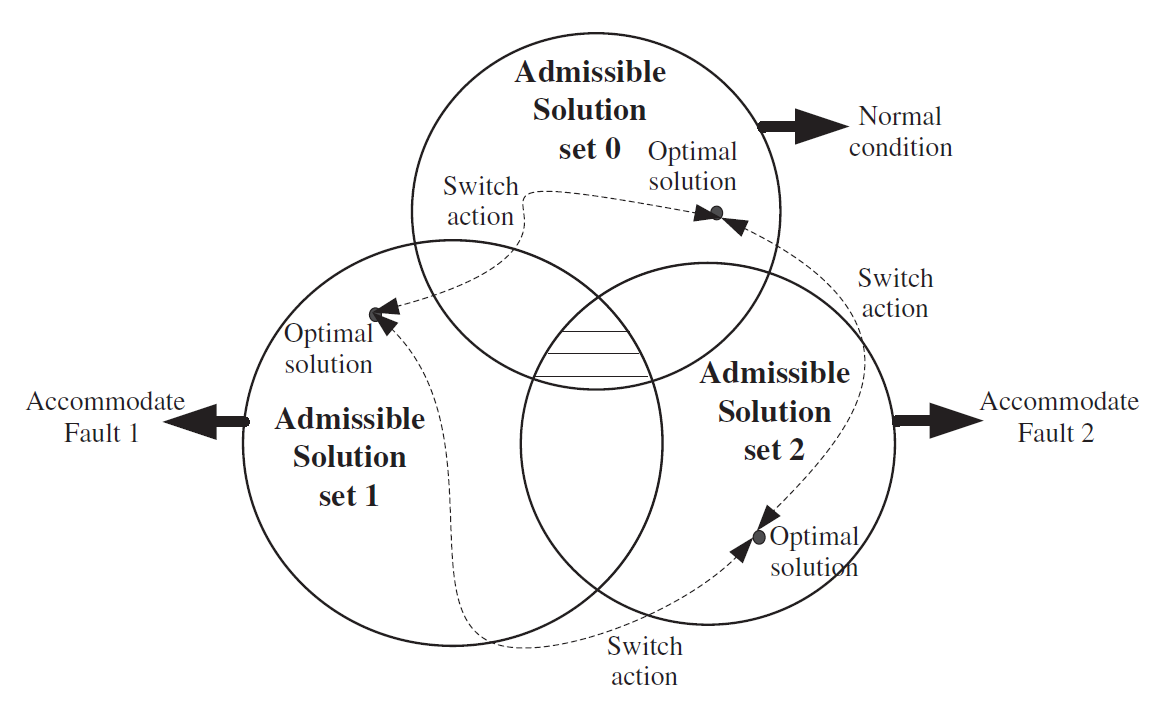
\includegraphics[width = 0.6\textwidth]{admissiblesp.png}
    \caption{可接受的控制空间示意\cite{Jiang201260}}
    \label{fig:asp}
\end{figure}
\begin{figure}[!htp]
    \centering
    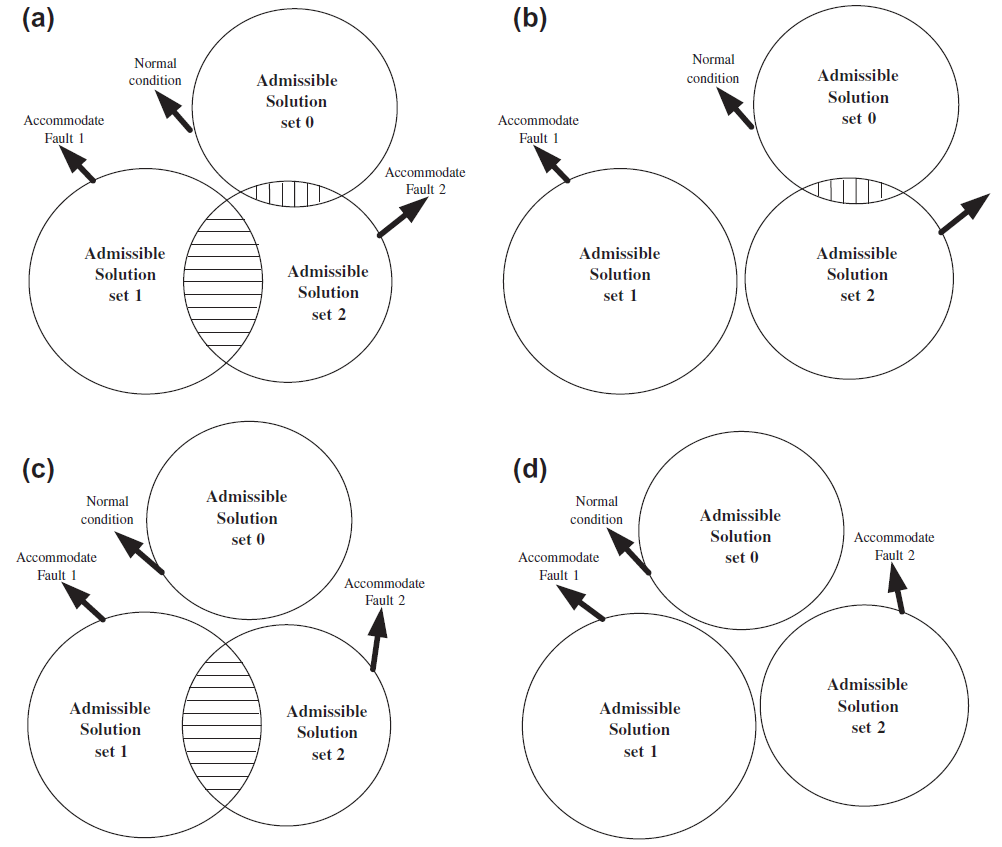
\includegraphics[width = 0.6\textwidth]{aspoverlap.png}
    \caption{其他控制器空间示意\cite{Jiang201260}}
    \label{fig:aspoverlap}
\end{figure}

\subsubsection{被动容错控制的发展}
被动容错控制文献中被称为可靠控制(Reliable control)。“可靠”的概念第一次由Siljak于1980年提出\cite{siljak1980},经过Date和Cho等人的发展\cite{70346,4790503},最终在1992年由Robert J. Veillette进行系统地总结\cite{119629},提出了“可靠控制”这一概念。往后,文献中的凡是以被动容错控制思路设计的控制器,都以reliable control呈现。

被动容错控制的设计方法有很多种,在$H_\infty$优化\cite{119629,7850999}、LMI方法\cite{7795198,974340,1236798}、LQ方法\cite{VEILLETTE1995137,847106,866928},滑模控制方法\cite{4160860},模糊系统\cite{7795198,7505963,Zha20173267},动态预补偿结合特征结构配置\cite{Jiang2000Design,ZHAO19981267},去中心化观测器\cite{70346}等方面均有相关研究成果。其中文献\cite{ZHAO19981267}首次给控制器冗余和错误构建了数学模型。另外,根据针对系统错误的不同,被动容错控制还可以分为针对执行机构失效\cite{ZHAO19981267,974340,VEILLETTE1995137,1236798,Tian20101907,Li20132455,7353144,7863042,70346,866928}、时变错误\cite{7850999,CHEN2004349,6064886}和随机错误\cite{7795198,7505963,5540530,Zha20173267}。

国内外也有不少文献对被动容错控制提出了分类方法。国外文献中,Fekih\cite{6859271}用鲁棒控制的分类方法把被动容错控制分为了数量反馈理论法、$H_\infty$范数优化法\cite{4079591}、LQ控制法\cite{Staroswiecki20072070}、$\mu$同步法和变结构方法。国内文献中,王德军\cite{wangdejun2014}、许德智\cite{xudezhi2013}和高志峰\cite{gaozhifeng2011}都将被动容错控制分为可靠镇定、完整性与联立镇定三类方法。肖冰\cite{xiaobing2014}认为在航天器姿态控制中,被动容错控制可以与主动容错控制的控制器重构部分做为一个方向共同研究。他将航天器姿态容错控制方法,分为基于自适应技术(Adaptive)的方法、基于滑模控制的方法和基于控制分配的方法三类,这一点在Yin. S的论文中\cite{7407616}也得到了有力的支撑。

\subsection{故障检测与诊断}\label{subsec:fdd}
故障检测(Fault Detection)与故障诊断(Fault Diagnosis)是两个不同的概念。故障检测,一般指系统对是否发生故障进行在线检测;而故障诊断,指的是在检测到故障的基础上,判断故障的类型和严重性。故障检测与诊断是主动容错控制器设计前的必经步骤。目前已经有很多综述文章阐述了故障检测与诊断的研究现状\cite{Venkatasubramanian2003293,6859271,Zhang2008229,7407616,6423903,Marzat2012modelbased,Jiang201260,5282515,Venkatasubramanian2003293,Venkatasubramanian2003A}。其中具体对故障检测的分类也有一些不同。

Inseok Hwang\cite{5282515}在文献中将故障检测分为硬件冗余(Hardware Redundancy)和分析冗余(Analytical Redundancy)两类。而其中硬件冗余主要是设计多传感器来尽可能明确地检测故障,可分为交叉频道监控(Cross channel monitoring, CCM)、残差生成(Residual Generation)和信号处理(Signal Processing)方法;分析冗余主要是用数学模型直接对系统当前状况进行估计,不需要多余的硬件,因此也更高效,分析冗余又可分为定性(Qualitative)方法和定量(Quantitative)方法。 Fekih\cite{6859271}认为所有故障检测都由三个步骤构成:残差生成(Residual Generation)、残差评估(Residual Evaluation)和最终判断(Decision Making)。在此基础上,诊断方法可以分为基于模型(Model-Based)的方法和不基于模型(Model-Free)的方法。其中基于模型的方法有模糊、神经网络、专家系统等方法\cite{Patan2008Artificial},不基于模型的方法主要是基于算法和统计的手段。Yin\cite{7407616}的文献中把故障检测分为两大类——基于模型的方法和基于数据的方法。其中基于模型的方法依赖于系统模型,而当模型不准确时,可以使用纯数据方法。

本文的观点与Fekih\cite{6859271}和Yin\cite{7407616}各有相似之处,认为不论基于模型还是数据,故障检测的思路都是通过设计一个残差函数来对故障进行判断,具体在残差函数的设计思路及依赖上,才有了基于模型、不基于模型或是基于数据的区别。因此,本文仍将故障检测的方法分为基于模型的方法和基于数据的方法。

\subsubsection{基于模型的方法}\label{subsubsec:modelbased}
对于基于模型的方法,文献\cite{Marzat2012modelbased}做了很好的综述。Venkatasubramanian的两篇综述\cite{Venkatasubramanian2003293,Venkatasubramanian2003A}将基于模型的故障检测分为定性方法和定量方法。通常来说,该类故障检测分为残差生成、残差评估两个环节\cite{Marzat2012modelbased},系统框图如图\ref{fig:FDDProcess}所示。在残差生成环节,使用系统的执行器输入和传感器数据来预测系统接下来的行为;然后将预测行为与系统实际行为进行比较。这里介绍几种基于模型的方法。
\begin{figure}[htp]
    \centering
    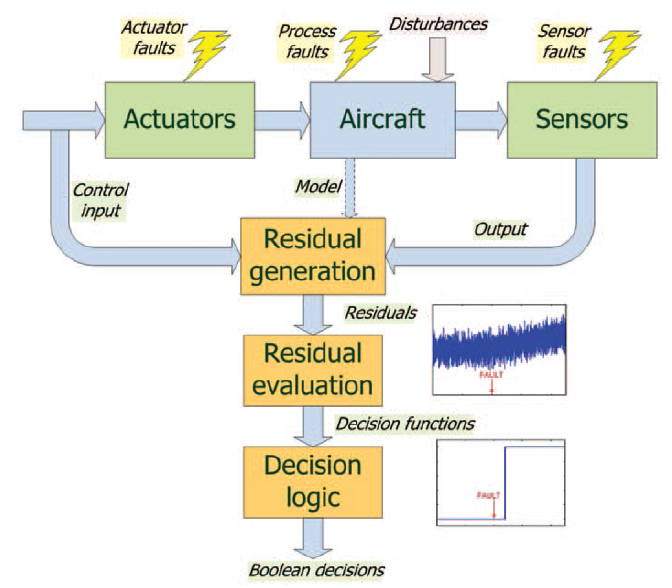
\includegraphics[width = 0.6\textwidth]{FDDProcess.png}
    \caption{一种典型的故障检测机制}
    \label{fig:FDDProcess}
\end{figure}
\paragraph{参数估计类方法}由于系统方程中的参数很可能没有直接的物理意义,而有些能测量到的物理量又不能明显地给出系统是否有错误的判断,参数估计故障诊断方法就是在这种背景下产生的。这类方法的思路是:把系统方程中的参数$\theta$与系统中具有实际物理意义但不能测量到的变量$p_a$(如舵偏角等)建立方程$\theta = g_p(p_a)$,然后首先依据系统观测方程$y=h(u,\theta)$测量到的$y$对参数$\theta$进行估计,得到$\hat{\theta}$;再通过$p_{a0} = g_p^{-1}(\hat{\theta})$求出可能的$p_{a0}$。最后将得到的$p_{a0}$输入事先设计好的残差函数,与事先设置好的可接受的$p_a$值进行比较。这是一种比较经典的方法,文献多在2000年以前出现\cite{ISERMANN1984387,FRANK1990459,ISERMANN1993815,411478,BLOCH19951709},其中对参数$\hat{\theta}$的辨识也成为了新的研究方向\cite{ISERMANN1993815,411478,BLOCH19951709},涉及到的方法多为最小二乘、卡尔曼滤波等一些最优估计的方法。参数估计的计算强度较大是这类方法的缺点,文献\cite{Villemonteix2009Bayesian}对参数估计提出了一种贝叶斯(Bayesian)优化方法。在残差函数的设计中,也可以设置多个可接受的$p_a$值的集合,详见文献\cite{Kieffer2011Guaranteed,Puig2010Fault}。

\paragraph{状态估计类方法}状态估计类方法的思路是通过对系统状态的估计与传感器测量的数据做对比,得到系统是否发生错误的判决。通常可以根据对不确定性的处理分为确定性方法、随机方法和有界误差方法\cite{Marzat2012modelbased}。

确定性方法\cite{1098323,ALCORTAGARCIA1997663}不考虑系统的误差和扰动,直接在模型中推导观测误差与错误的关系。Luenberger观测器\cite{1098323}是这种方法第一次被应用到线性系统上。由于非线性系统线性化的时候会产生误差,因此又有了处理非线性系统的扩展Luenberger观测器(Extended
Luenberger Observer, ELO)\cite{Nejjari2008Extended,ZEITZ1987149}。此外,由于非线性系统的复杂性,也有很多种观测器得到了研究,如自适应观测器(Adaptive observers)\cite{878691,Zhang2010290}、高增益观测器(High-gain observers)\cite{Busvelle2002HIGH}、滑模观测器(Sliding Mode Observers)\cite{Edwards2011Sliding,1269645}和基于偏微分方程(partial-differential equation)设计的新型观测器\cite{5717995}。

随机方法中,通常假定系统的噪声扰动服从高斯分布(Gaussian Distribution),在处理线性系统时以卡尔曼滤波器(Kalman Filter)为代表。基于卡尔曼滤波器的容错方法首先在文献\cite{MEHRA1971637}中提到,而后\cite{NIKOUKHAH19941851,539440,willsky1986detection}做了后续延伸工作。处理非线性系统时,有扩展卡尔曼滤波(Extended Kalman Filter, EKF)、无迹卡尔曼滤波(Unscented Kalman Filter, UKF)和粒子滤波(Particle Filter, PF)。扩展卡尔曼滤波通过对非线性系统线性化来使用卡尔曼滤波\cite{CHANG19952861};无迹卡尔曼滤波则不对系统线性化,通过一些系统状态采样点来逼近系统状态的高斯分布\cite{4252507,XIONG2005113}。粒子滤波则可适用于非线性非高斯分布的噪声,它采用蒙特卡洛方法对错误进行建模并估计\cite{1271398,971661}。

有界误差方法不同与上面两种。上面两种都使用了显示的故障模型或概率分布,而有界误差方法使用故障的上界进行处理。这类方法的文献如区间分析法\cite{4547434}和神经-模糊方法\cite{Korbicz2007609}。

\paragraph{奇偶校验空间法}奇偶空间校验(Parity Space)方法比较容易从直观上理解,是一种解除系统状态和错误之间的耦合,从而方便设计出只跟故障有关的残差函数\cite{patton1991review,GERTLER1995627}。具体来说,对于一个静态线性观测系统:
\begin{equation*}
    \mathbf{y} = \mathbf{Cx} + \mathbf{E_fw_f}
\end{equation*}
其中$\mathbf{w_f}$是系统错误,$\mathbf{y}$是观测变量。此时如果设计一个矩阵$\mathbf{W}$,使得$\mathbf{WC=0}$,那么残差函数$\mathbf{Wy}$就只与系统错误$\mathbf{w_f}$有关了,可以依次设计残差函数。对于动态系统,可以用\cite{Marzat2012modelbased}中提及的方法先把系统化成静态系统的形式。对于非线性系统,则可以用线性化、仿射变换等方式来处理,详见文献\cite{Staroswiecki2001687,shumsky2007redundancy,1024022,948476}。

\paragraph{去耦合类方法}在故障检测设计残差函数时,经常遇到的一个问题是如何区分系统的正常扰动和意外故障。一个理想的残差函数应该满足:1)只对系统错误有响应,对系统状态和扰动无响应;2)在系统没有故障的时候,能够随着时间的推移收敛到0\cite{1104419}。这里介绍四种去耦合类的方法。

第一种是特征结构分配的方法\cite{261546}。该方法给系统的输出估计偏差$\mathbf{e_y}$左乘了一个权值矩阵$\mathbf{W}$作为残差函数\cite{261546,RNC:RNC523}。同样的方法也可以用在奇偶校验空间的残差设计中,使得残差对系统扰动不敏感\cite{doi:10.1080/00207179508921908}。

第二种是未知输入观测器(Unknown-input Observer, UIO)。这种观测器能够在估计系统状态的同时将外部扰动的影响降到最小\cite{jie1996design,1657536,220921}。简单将未知输入观测器的原理说明如下,假设系统如\eqref{eq:UIO1}所示。
\begin{equation}\label{eq:UIO1}
\begin{cases}
\dot{x} = Ax+Bu+E_dw_d+E_fw_f \\
y = Cx 
\end{cases}
\end{equation}
其中$w_d$代表扰动,$w_f$代表错误。针对该系统的位置输入观测器设计如\eqref{eq:UIO2}所示
\begin{equation}\label{eq:UIO2}
\begin{cases}
\dot{\hat{x}}=F\hat{x}+TBu+(K_1+K_2)y \\
\mathbf{r} = (I-CH)y-C\hat{x}
\end{cases}
\end{equation}
其中,$\mathbf{r}$为残差函数,$F,T,K_1,K_2,H$都是设计参数,需满足以下条件:
\begin{equation*}
\begin{cases}
(HC-I)E_d=0\\
T = I - HC\\
F= I-HCA-K_1C\\
K_2=FH
\end{cases}
\end{equation*}
只要这样的观测器存在,那么可以用\cite{4101989}中提及的DOS(Dedicated observer scheme)或者GOS(General observer scheme)的方法进行故障检测系统设计。

第三类方法是$H_{\infty}$方法。这种策略适合精确解耦无法达到的情况\cite{doi:10.1080/002071799220704,Henry2005251}。$H_{\infty}$方法的思想是,根据$H_{\infty}$范数设计残差函数,使得错误对其影响最大,并且扰动对其影响最小。运用线性矩阵不等式(Linear Matrix Inequality, LMI)是解决这类问题的标准化方法\cite{Zhong2003543}。

第四类是非线性几何方法。微分几何的方法\cite{928586,Bokor2009113}能够检测是否存在一个只对一种错误敏感的滤波器\cite{Marzat2012modelbased}。微分代数的方法也有文献,如\cite{berdjag:hal-00198435}。此外,还有一种逆向的方法\cite{edelmayer2004input,doi:10.1080/00207170802582215,1102181}。该种方法不同于大多数故障检测方法。大多数故障检测系统都使用估计系统输出与测量到的系统输出作比较或设计残差函数,这种逆向方法使用系统输入与前一时段发送给系统执行器的输入作比较。由于大多数飞行器都装备了惯性测量元件(Inertia Measurement Unit, IMU),针对利用惯性测量元件的故障检测也有相关文献\cite{MARZAT2010951,5676073}。

\paragraph{闭环方法}前面介绍的几种故障检测方法都是未考虑反馈控制的开环检测方法。但事实上控制信息能极大地辅助故障检测。比如设计一个辅助控制器添加到系统本身的输入中\cite{NIEMANN2006587,ASHARI2009192}。文献\cite{ASHARI2009192,4602147}将这种方法应用到无人机上,通过添加一个微小的正弦控制量的方法进行故障检测。但是这种方法需要非常小心,需要保证添加的控制量不会严重干扰系统的稳定性和表现\cite{Niemann2006Active}。

鉴于以上原因,闭环方法需要在控制表现和故障检测能力中做取舍。Jacobson\cite{92987}设计了同时能够控制和故障检测的模型。 相关的多目标优化问题也成为了研究的热点。Henry\cite{Henry2005251}提出了一种对这类问题的建模,并用线性矩阵不等式得到了问题的最优解。Niemann\cite{649678}对闭环故障检测方法的效果与开环方法做了对比。

\subsubsection{基于数据的方法}\label{subsubsec:databased}
基于数据的方法又可以称为不依靠模型的(Model-Free)方法。Yin在基于数据的方法有较多的研究文献\cite{6717991,7394158,7067026,6748057,7297846,7407616}。其中文献\cite{6717991,6748057,7407616}提供了基于数据的故障诊断的文献综述。基于数据的方法特点是,容错控制器的设计完全不考虑

\subsection{主动容错控制}\label{subsec:active}
主动容错控制的思想是通过在线辨识系统控制设备的状态,估计控制器的错误类型,并针对已发生的错误种类,实时生成能够让系统继续保持稳定的控制器。主动容错控制系统一般分为两个步骤:故障检测以及控制器生成。故障检测又可分为两大类——基于模型和不基于模型的;控制器生成可以分为三大类——控制器池法,控制分配方法

\subsubsection{基于控制分配的容错控制}
通常,一个有冗余的控制器可以建模如\eqref{eq:adundantnonmodel}
\begin{equation}\label{eq:adundantnonmodel}
\tau = h(u,x,t)
\end{equation}
其中$h$是控制器函数,$\tau \in \mathbb{R}^m$,$u\in \mathbb{U} \subset \mathbb{R}^p$ 是控制输入,而$\mathbb{U}$代表控制器的取值空间,$\mathbb{R}^p$代表$p$维线性空间。控制分配方法的主要思想是通过安置冗余的控制器或传感器,在一个或多个设备出现故障的时候(即$u$无法达到期望取值的时候),及时调整控制器的输入$u$,使得控制器的输出$\tau$维持不变或变动很小。鉴于控制器设计的时候留有冗余,因此通常情况下有$p>m$。
\subsubsection{第二类主动容错}
\subsubsection{第三类主动容错}
\subsubsection{第四类主动容错}
\subsection{飞行器容错}\label{subsec:aircraftftc}



\section{研究方法}
\subsection{拟解决的关键问题}
\subsection{现有的研究手段}
\subsection{问题的难点}

\section{论文目录}

\bibliographystyle{unsrt}
\bibliography{MyBib_Control}

\end{document}
